%%%%%%%%%%%%%%%%%%%%%%%%%%%%%%%%%%%%%%%%%%%%%%%%%%%%%%%%%%%%%%%%%%%%%%%%%%%%%%%
\subsection{Characteristics of Bees}
\label{subsubsec:bees}
%%%%%%%%%%%%%%%%%%%%%%%%%%%%%%%%%%%%%%%%%%%%%%%%%%%%%%%%%%%%%%%%%%%%%%%%%%%%%%%
For snapshot~3, I inspected the properties of each honey bee, concerning its degree~$k$, strength~$s$, local clustering coefficient~(lcc)~$c$, betweenness centrality~$C_B$ and closeness centrality~$C_C$ and derived charctersitics and properties of the honey bee colony.

\subsubsection{Low Hierarchical Structure}
The degree is normally distributed (a in figure~\ref{fig:n3-degreeStrLCC}).
Therefore most bees bee have the same high number of interaction partners.
The absence of hubs, a small number of highly connected bees, indicates a low hierarchical structure of the network.
Strength and lcc are also normally distributed (d and g in figure~\ref{fig:n3-degreeStrLCC}).
That also shows the absence of extreme values and confirms that bees are similar to each other regarding those properties.
Betweenness and closeness centrality (j and m in figure~\ref{fig:n3-degreeStrLCC}) also follow a normal distribution.
This leading to the assumption that no central or important bees exist.
All bees are similarly close to all other bees in the network, and every bee can reach any other bee with a few steps.
That also corresponds to the low average path length, and the small diameter of the network described in section~\ref{subsec:colony}.
The absence of bees with a high betweenness suggests that the colonies functionality is robust concerning the disappearance of single individuals.

\subsubsection{Correlation of Local Network Measures and Detection Frequency}
Degree, strength, closeness and betweenness (b, e, k, and n in figure~\ref{fig:n3-degreeStrLCC}) show a positive correlated with the detection frequency. A low value corresponds to a low detection frequency. In contrast, the local clustering coefficient (h in figure~\ref{fig:n3-degreeStrLCC}) and detection frequency are negatively correlated.

\subsubsection{Some Groups}
[TODO: überarbeiten! manche Bienen treten zwar an diesem Tag ihren Dienst an, sterben aber anscheinend während der Arbeit, da es nur wenige alte Bienen sind, wird der Mean sehr verfälscht]\\

The histograms of degree, strength, betweenness, and closeness show a tendency for multimodality, indicating the presence of some bee groups. The local clustering coefficient distribution is rather right skewed, with one peak at $0.75$

There is no clear boundary between groups in the degree distribution plot (a), but a value around 0.4 can be estimated.
The strength histogram (d) seems to have a border at a strength of 1000.
For closeness (j) and betweenness (m), a border can be seen at 0.6 and 0.0001.
All distributions indicate a small group (~100 bees) and a second larger group containing the rest of the colony.

The first small group interacts on average with 20\% of the colony and has a very low strength (number of total interactions below 250). The closeness value is compared to the second group smaller but still over 0.5. The betweenness has a small range and is close to 0 for the first smaller group.
The second group interacts with about 80\% of the colony, corresponding to almost the entire colony and an average strength of 5000. A high strength can result from lots of neighbors with low edge weights or a few neighbors with high edge weight. The second is rather unlikely, looking at the edge weight distribution (figure~\ref{fig:edgeWdist}). The second group is characterized by a very high closeness (0.75) and a still very low betweenness but higher than the first group (0.0005).

All age-correlation plot show a seperate group of bees older than 45 days, seeming to correspond to the first smaller group of bees described above.
This older group is characterized by a low degree, a low strength, and low closeness and betweenness. In contrast, a high lcc, compared to the younger group is noticeable.
The younger group relates to a high degree and strength, as well as a high betweeness and closeness compared to the first group, but a lower lcc.
A high lcc of the old group indicates a high connection within the younger group and only less connectivity between bees of the older group.


\begin{figure}[!h]
	\centering
	\begin{subfigure}[b]{1.0\textwidth}
	\centering
	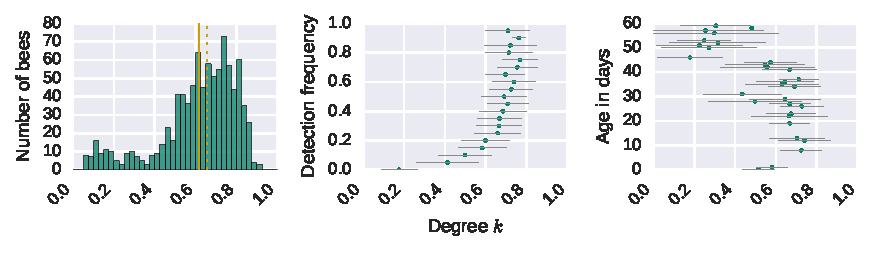
\includegraphics[width=1.0\textwidth]{Figures/n3-stat-degreeAgeDetF.pdf}
	%\caption[Degree]{\textbf{Degree}}
	%\label{fig:n3-degree}
	\end{subfigure}
	\begin{subfigure}[b]{1.0\textwidth}
	\centering
	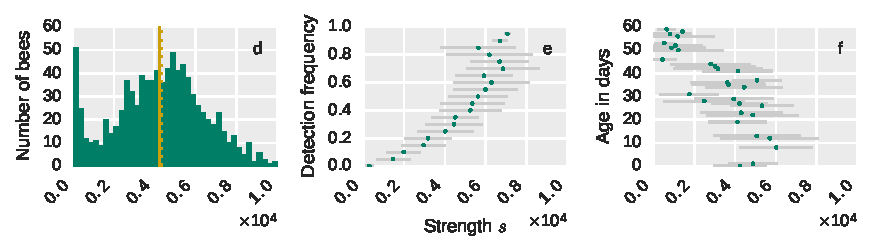
\includegraphics[width=1.0\textwidth]{Figures/n3-stat-strengthAgeDetF.pdf}
	%\caption[Strength]{\textbf{Strength}}
	%\label{fig:n3-strength}
	\end{subfigure}
	\begin{subfigure}[b]{1.0\textwidth}
	\centering
	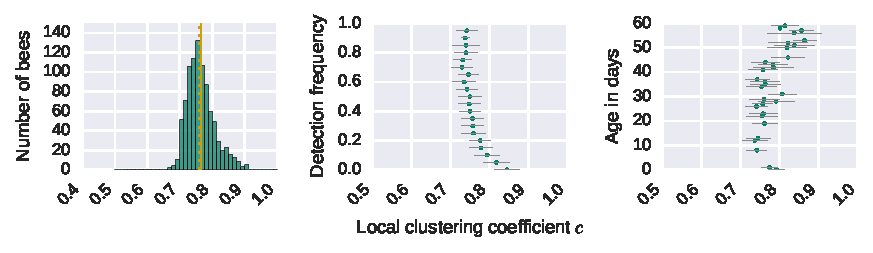
\includegraphics[width=1.0\textwidth]{Figures/n3-stat-lccAgeDetF.pdf}
	%\caption[Local clustering coefficient]{\textbf{Local clustering coefficient}}
	%\label{fig:n3-lcc}
	\end{subfigure}
	\begin{subfigure}[b]{1.0\textwidth}
	\centering
	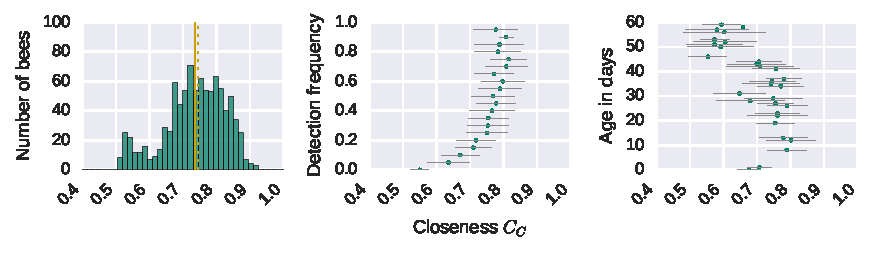
\includegraphics[width=1.0\textwidth]{Figures/n3-stat-closenessAgeDetF.pdf}
	%\caption[Closeness Centrality]{\textbf{Closeness Centrality}}
	%\label{fig:n3-closeness}
	\end{subfigure}
	\begin{subfigure}[b]{1.0\textwidth}
	\centering
	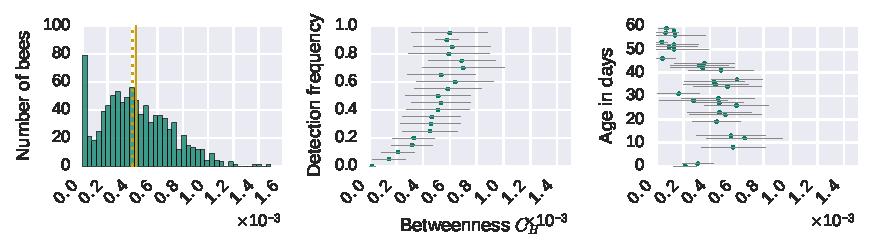
\includegraphics[width=1.0\textwidth]{Figures/n3-stat-betweenAgeDetF.pdf}
	%\caption[Betweeness Centrality]{\textbf{Betweeness Centrality}}
	%\label{fig:n3-between}
	\end{subfigure}
	\caption[Local measures in relation to age and detection frequency]{\textbf{Local measures in relation to age and detection frequency}}
	\label{fig:n3-degreeStrLCC}
\end{figure}